\chapter{Architecture 1.0}
%Lines:HTML
%	177 pom
%+	3859 api java
%+	1937
%+	305
%+	1668
%+	110
%+	426
%+	262 pom
%+	1159 jsp java
%+	2633
%+	265 xml
%+	116
%+	47
%+	2903
%=	15867

	
\section{Introduction}
In this chapter we look at the architectural details of Architecture 1.0, which is an implementation of Shredhub that conforms to \textit{Reference-model 1.0}. The application is written in Java, and uses the SpringMVC framework. I could have chosen to use another technology like Ruby on Rails, Sinatra for Ruby or a Microsoft .NET framework, considering these are all very popular Web application environments. However, because I happen to know the Java programming language very well, choosing a Java-based Web framework was preferable. Although there are other Java-based Web frameworks in addition to Spring, Spring was chosen because it is very easy to set up, it provides a wide collection of plugin extensions, and most importantly, for the relevance of this thesis, it is one of the most popular Java-based Web frameworks \cite{popFrameworks}.

The application runs on Apache Tomcat, which serves as both a Web server, and an application server. The database is implemented with PostgreSQL. It runs on a database server which for simplicity is deployed on the same physical machine as Tomcat. Here I could also have chosen a different database technology, for instance MySQL or Oracle SQL. However, I chose PostgreSQL because I have experience with the technology, it also has a lot of good and available documentation, and it is a very popular database choice for modern Web applications\cite{popularDB}.


In the following sections we look into the implementation details of the source code. We discuss the problems that occurred along the way, choices that were made, and potential alternative solutions. The discussion is divided into three; one part for each software layer in the application.


\section{Architectural Overview}
%\begin{wrapfigure}{r}{0.5\textwidth}
%  \begin{center}
 %   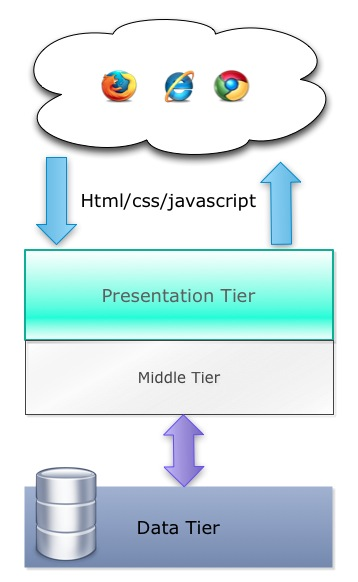
\includegraphics[width=0.48\textwidth]{images/architecture1.jpg}
 % \end{center}
 % \caption{Overal architecture 1.0}  \label{fig:architecture1}
%\end{wrapfigure}

Architecture 1.0 is a back-end-oriented application. All of the application's logic happens in a Web application that runs on an Apache Tomcat server. In respect to \textit{Reference-model 1.0}, the application is separated into three software layers with different responsibilities; a presentation layer, a domain logic layer, and a data source layer. I have chosen this separation of concerns in order to facilitate application maintainability and flexibility. I could have chosen to implement everything in two, or even one layer, but this would resolve in classes having very many responsibilities, and tight couplings. 

The Web app depends heavily on HTTP sessions to maintain user-state. When a user enters www.Shredhub.com, SpringMVC generates an object (called the HTTPSession object) who's lifetime lasts throughout the user's session. This object is used as a container for storing state information.

The application's front-end consists of a set of HTML templates that we refer to as \textbf{views}. The views are implemented with the JSP template language technology, and are turned into HTML pages by a template rendering engine, provided by Spring. The client user primarily communicates with the application through three different interaction schemes: 
\begin{enumerate}
\item {} Hyperlinks
\item{} HTML forms
\item{} Buttons or text input-fields that are picked up by JavaScript handlers
\end{enumerate}
For all of the different user-interaction schemes in listing 1 and 2, there will be a corresponding controller handler on the backend. These actions always result in a new view being rendered and returned to the client. Interaction scheme 3 only occurs a few times on the application, in special cases that require highly responsive behavior, in which a server round-trip must be avoided. This is managed by AJAX calls that are implemented inside the views. 

% \begin{figure}[h]
%  \centering
%  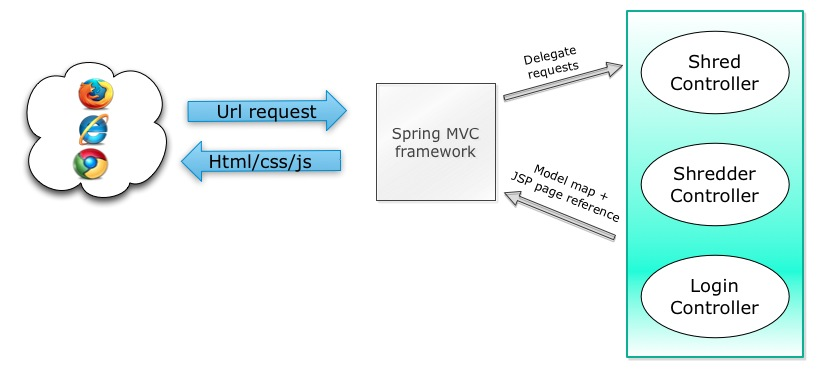
\includegraphics[scale=0.5]{images/presentationtier1.jpg}
%  \caption[sp.]
%   {The presentation tier's responsibility }
%    \label{fig:presentationtier1}
%\end{figure}
\section{The Presentation Layer}
The presentation layer is the first entry point in the application. Its responsibility is to handle client interactions, meaning it will handle authentication, state and session management, and input validation. It is built with the model-view-controller pattern. This decision  was made because the structure is familiar to many Web developers, and it neatly separates concerns into coherent and decoupled classes.  

\subsection{Authentication}
Users must to be authenticated in order to use any of the pages on Shredhub except the login page. Most of the authentication and access control handling is set up to be handled automatically by Spring. For simplicity, I have chosen to use an HTML form-based authentication mechanism that relies on a username, password and security-role. Other common authentication solutions used in Web apps are HTTP BASIC or HTTP Digest, or HTTP X.509 client certificate exchange. However, I find that form-based authentication fits the simple scope that has been chosen for authentication in this thesis, and it conforms to \textit{Reference-model 1.0}, because it relies on the server-side sessions.

The form based authentication process works by letting users enter a username and password in an HTML form on the login page. On form submit, the request is picked up by Spring, which will look in the database for a Shredder with the given username, password. The database row for a Shredder also contains a column that represents the Shredder's user-security-role. However, for simplicity there is only one role in this application , which is the one that gives access to everything. If a row with a matching username and password is found, the framework will grant access to the user, and the user will now have access to the whole Web app. To avoid having to re-authenticate for every subsequent request, Spring will behind the scenes maintain a security-context object that is connected to the user's HTTPSession. The security-context object simply indicates that the user has successfully logged in once, and is allowed to perform the given request. 
		  
\subsection{State and Session Management}
The presentation layer is responsible for managing state associated with a user when he navigates around the application. In Architecture 1.0, this is implemented by using Spring's HTTPSession object. Now, considering that Spring offers readily available in-memory objects scoped at session-level, makes it very appropriate to use such objects as caches for data that is frequently accessed. State data is put either in objects that are maintained by the IOC container and scoped at session-level, or directly on the HTTPSession object, using a method called \textit{setAttribute(String key, Object value)}. The separation is a matter of separation of concerns; HTTPSession objects maintain meta data concerning the user (profile info, battle requests, battles, fanees etc), while other session-scoped objects maintains data regarding the user's page activities (e.g current shred-row, current shredder-page etc).

 Data that is used to populate views on the server has to be fetched from the database. Many of these database calls can be avoided if some of the data is stored in memory. The data could for instance be a particular set of Shreds that must be fetched especially quick in order to achieve responsive behavior, user data that is displayed often, e.g the user's name, or a list of battle requests which is meant to be visible on the top navigation-bar at all time. The problem however, is that there is a tradeoff in how much data should be kept in memory, as maintaing too much memory turned out to make the application slow, and in worst case lead to out-of-memory- exceptions. Also, and this is a special case for typical Web 2.0 applications, data tend to change frequently, and users naturally want up-to-date views of the data. Therefore, content regarding the Shreds and the newest Shredders on Shredhub, new fan-connections and other data that frequently changes, for simplicity shouldn't be cached. However, alternative solutions that makes it possible to cache such data is to some extend possible, for example by implementing push-based public-subscribe service that signals the cache to update whenever an update is made. Or alternatively a pull based solution where some service frequently pulls the database for new updates. Unfortunately, because of lack of time for this thesis, such solutions have not been implemented.

The set of Shreds that are displayed in the shred-pool are partly being cached in memory: the shred-pool is made up of multiple rows of Shreds. Each row consists of 3-5 Shreds, depending on which Shred-row it is, and the user can click a next button in order to change the current row to a new set of Shreds. Now, for each row, the server fetches a set of 20 Shreds from the database, and maintains these in a session-scoped cache. Whenever the user clicks on the ``next'' button in a row, the server checks the cache for that row to see if the next row of Shreds lies within. If they do, the row is moved one row-size, and this new row of Shreds are displayed. If not, the server fetches another 20 Shreds from the database, puts them in the cache, and displays the first new row. This way, the server avoids many calls to the server, which is very important in order to get quick and responsive behavior when the user clicks the next button. The cache could also be bigger, but then again there is a tradeoff in how big the cache can be without influencing performance. 

\subsection{Input Validation}
Input validation is both part of the presentation layer, which addresses form-input rules, and the domain logic layer, which enforces business rules of the input data. In the presentation layer, validation is usually the first thing that happens once a URL request enters the server. Validation is always performed by applying positive filtering, meaning I specify what is allowed, and forbid everything else. Another approach is to do negative filtering where the input is scanned for illegal patterns. However the latter approach is not as secure because it is hard to imagine all possible attack-forms\cite{sqlinjection}. Also, new forms of attacks might be invented in the future. However, positive filtering has the downside that it might be to restrictive.

The controller handlers and interception filters validate HTML forms, and the controllers often check that the user stored in the session is allowed to perform a given business operation. 

\subsection{Controllers}
Controllers are first-class citizens in the presentation layer, who's responsible for processing URL requests. Controllers are Java classes that are mapped to a specific URL pattern. A simple approach is to have one controller class that is used for every URL supported by the Web app. However, this is not very maintainable, as the class would  grow exceptionally large, and have many responsibilities. Other solutions are for instance to have one controller class for every view, or one for every domain object. I have chosen to implement something in between. I chose to implement one controller class for each main resource/domain in the application, in addition to one controller for the home and Shredpool view (simply called the Logincontroller). In table ~\ref{table:controllers} below we can see all the controllers in Architecture 1.0, together with some example controller handlers and their respective responsibilities. Although not displayed in the table, each controller handler is mapped to a unique URL. The controller's main responsibility is to delegate control to a proper business operation in the domain logic layer. 


\begin{table}
\centering
    \begin{tabular}{ |  l  | p{6cm} | p{3.5cm} |}
    \hline
	\textbf{controller handler} & \textbf{Responsibility} & \textbf{view returned} \\ \hline    
    \multicolumn{3}{|c|}{HomeController} \\ \hline
    loginPage() & Handles requests for the login page. Fetches the top-rated Shreds from the database and renders the login page & The login view \\ \hline    
    
    loginSuccess() & Called when authenticating the user succeeds. Populates the session cache with data fetched from the database & Redirects to the shred-pool \\ \hline
    
    theShredPool() & Fetches from the database the set of Shreds and all the shred-news that are to be displayed in the shred-pool. & The shred-pool view \\ \hline    \multicolumn{3}{|c|}{ShredController} \\  \hline
   
     createShred() & Creates a new Shred and saves it in the database & The shred-pool \\ \hline

     postComment() & AJAX supported function that given a shredId and comment-text, adds a new comment to a Shred where the comment-owner is set to the id of the user (stored in session) & None, AJAX request \\ \hline
     
    \multicolumn{3}{|c|}{ShredderController} \\      \hline
getShredders() & Fetches the next page of 20 Shredders that are to be displayed in the list of Shredders view. The page number is maintained in the session object & The shredders view\\ \hline
followShredder() & Adds a new fanee to the user's list of fanees. Updates the session-cached list of fanees for the user  & The shredders view \\ \hline

 \multicolumn{3}{|c|}{BattleController} \\ \hline
 getBattle() & Fetches a battle object given a Battle Id & The battle view \\ \hline

newBattle() & Called when a Shredder accepts a Battle request that is being kept on the session object. Creates a new Battle object. Stores it in the database & The shred-pool view \\ \hline
    \end{tabular}
    \caption{The set of controllers in Architecture 1.0}
    \label{table:controllers}
\end{table}

One big advantage with the three-layered architecture becomes clear here; if I choose to change the structure of the controllers, it would not affect the domain logic layer, because the domain logic layer does not depend on the presentation layer. A concrete example of the data flow in the presentation layer is given in section~\ref{sec:apres} in Appendix A.

 
\subsection{Views}
In this architecture, views are template files that are used to dynamically generate HTML. These views are implemented with the Java Server Pages (JSP) technology. Now, it is considered best practice to avoid implementing business logic in the views\cite{sepbiz}. View and Java logic in the controllers together cooperates to create view logic that dynamically generates a page depending on the current state, and user-input. To blend together business logic and view logic implementation would result in tight couplings between two very different concerns. This is one of the reasons I chose to implement the MVC pattern, because it nicely separates these concerns, making it easy to change the view without harming the business logic, and likewise to let the models be unaware of its presentation, so the models and their presentation can change independently.

\subsubsection{Main Components}
There is one view for each page in Shredhub. These are:
\begin{enumerate}
\item{} The login view
\item{} The shred-pool view
\item{} The shredders view
\item{} The shredder view
\item{} The Battle view
\end{enumerate}

Also, there are some views that are re-used in the above views:
\begin{enumerate}
\item{} The header view
\item{} The footer view
\item{} Show shred view
\end{enumerate}

Each of these views are implemented as a JSP file, e.g login.jsp. The last three views in the list are injected into the other views using special JSP syntax, in order to avoid view duplication. The views contain static HTML tags that never change, some AJAX functions written in JavaScript, and external links to CSS files and JavaScript libraries. JSP tags are used to inject the domain objects into the view by referencing to the model object that is populated with data in the controllers. The JSP implementation also has some if/else condition tags in order to generate pages given the current state of the application. 

When a controller handler finishes, a view is rendered and sent back to the client. Some view logic is also implemented with JavaScript inside the JSP files. In respect to \textit{Reference-model 1.0}, these are just self-contained and independent functions that has one single purpose, and therefore contains no particular architectural structure. An example of how view logic is implemented is given in section~\ref{sec:aview} in Appendix A. 

\subsection{Summary of The Presentation Layer}
The presentation layer is built with MVC. Form submits and link actions are picked up by a specific controller handler on the server. The handler performs validation, state management, and delegates to a business function in the domain logic layer.

Models are implemented in a lower layer, but are heavily used by the presentation layer. After a business operation is performed, the controllers are responsible for choosing which model objects to send to a view, which is rendered to HTML and sent back to the client.

The presentation layer depends heavily on the application's state that is implemented in session-scoped objects.
			
\section{The Domain Logic Layer}
The domain logic layer is the part of the application that receives a specific action from the controller, and performs the necessary business logic needed to complete the action. Now, since the responsibility of the logic layer is to implement the business logic in the application, it is important that this software layer is flexible. Flexibility, means that it can be relatively easy to add new features without harming anything else in the source code, and it should be easy to modify the already existing code. To achieve this, I needed a coherent design, preferably built with design patterns that gives a proper structure to the software architecture. To organize the layer, I have chosen to use the service layer design pattern\cite{poea}. With this implementation, each service represents the business operations that operates on a particular resource, or domain in Shredhub (e.g a Battle, a Shredder, or a Shred). However, this is not to be associated with the application's domain objects which concerns the domain resources' data, not functions. Instead, the service abstractions wraps the set of operations that are supported for each resource. Thus, each service class has a set of service functions. The list of service classes with some essential service functions are given below:
		\begin{enumerate}
			\item{} BattleService 
				\begin{itemize}
					\item{} getBattleWithId
					\item{} getOngoingBattlesForShredderWithId
					\item{} acceptBattleWithId
				\end{itemize}
			\item{} ShredderService
				\begin{itemize}
					\item{} addShredder
					\item{} getShredderWithId
				\end{itemize}	
			\item{} ShredNewsService
				\begin{itemize}
					\item{}getLatestShredNewsItems
				\end{itemize}
			\item{} RecommendationService
				\begin{itemize}
					\item{}getRecsBasedOnShreddersShredderMightKnow
				\end{itemize}
			\item{} ShredService
				\begin{itemize}
					\item{} getFanShreds
					\item{} getAllTags
					\item{} getShredsForShredderWithId
				\end{itemize}
		\end{enumerate}

\begin{figure}
		  \begin{center}
		\fbox{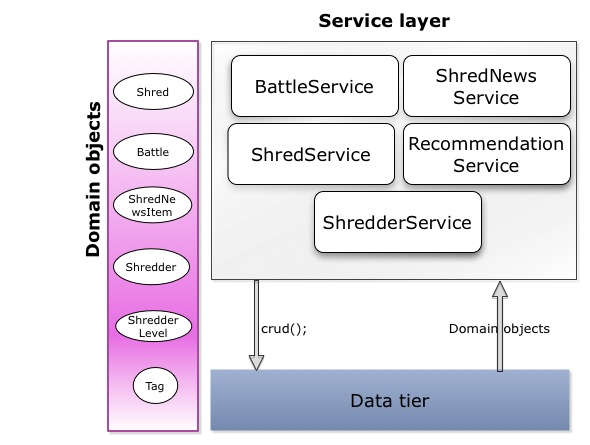
\includegraphics[width=\textwidth] {images/middletier.eps}}
		% Kommandoen \fbox tegner en ramme.
		\end{center}
		\caption{The domain logic layer and its connection to the datasource layer}\label{fig:middletier}
\end{figure}

\subsection{Service Functions and Domain Objects} 
An overview of the domain logic layer and its responsibility relative to the data source layer is given in figure \vref{fig:middletier}. The figure shows all the service abstractions, and the main domain objects in Architecture 1.0 (there are additional minor domain objects as well, such as ShredComment, ShredRating etc). The domain objects represent the application's core resources, implemented as simple Java classes with no logical functionality, just attributes with accessor methods. They can be seen to the left on the figure. These objects have references to each other, and are used across all three layers in the application, making them the one means for communicating the domain in the application. The logic layer sends and receives domain objects from the data source layer when they are to be manipulated in the database. 

An alternative architecture I could have chosen instead of the service layer pattern, is the transaction script pattern, but this is too simple for this application, and lacks structure. Another alternative is to use the domain model pattern. This is a good approach, but in this case, the domain objects would end up being very big, with lots of responsibility. I prefer the service layer pattern, because it decouples the operations from the object's state.

Most operations in the domain layer follow the same structure; some data is fetched from the datasource layer, this data is manipulated together with the data it got from the calling controller handler, and the result is written back to the database. Also, sometimes the newly updated data is returned back to the controller, so that this can be rendered in a new view. If an error occurred along the way (for instance if illegal data was sent from the controller), an exception is thrown and picked up by the controller so it can return an error view. An example of the data flow in the domain logic layer is given in section~\ref{sec:abiz} in Appendix A.

\subsection{Summary of The Domain Logic Layer}
The domain logic layer implements the domain of the application. The layer is divided into two; a service layer that implement business logic operations, and the domain objects which wraps the domain into self-contained data holders. The services forms a facade that is used by the controllers in the presentation layer. The services delegate to the data source layer for persistence.
	
\section{The Data Source Layer}
The datasource layer is the part of the application that receives a particular CRUD command from the domain logic layer, executes a SQL operation on the database, maps the result to a domain object and returns the result back to the business logic layer. The database is made with PostgreSQL. I have chosen not to use an ORM mapping tool, but rather build Java functions that talks directly to the database using Strings as queries, and mapping query results manually to Java objects. There are many good ORM technologies I could have chosen to use, for example Hibernate, and JPA, which would hide the complexity of serializing Java objects to SQL, and the opposite, and not having to deal with SQL. However, these technologies does not give me the control I need to debug and create flexible marshalling and queries. A tradeoff though, is that this tend to get messy, especially when the queries get many and complicated. I do however very much enjoy writing SQL queries. 
		
\subsection{SQL Implementation}
The SQL tables that represent the three central domain objects in the application is showed in the example below: 
		
\begin{lstlisting}[language=SQL]
	CREATE TABLE Shredder (
		Id				serial PRIMARY KEY, 
		username			varchar(40) NOT NULL UNIQUE,
		BirthDate			date NOT NULL CHECK (BirthDate > '1900-01-01'),
		Email				varchar(50) NOT NULL UNIQUE,
		Password			varchar(10) NOT NULL,
		Description			text,
		Address			text,
		TimeCreated		timestamp DEFAULT CURRENT_TIMESTAMP,
		ProfileImage		text,
		ExperiencePoints	int	DEFAULT (0),
		ShredderLevel		int DEFAULT (1),
		Guitars			text[],
		Equiptment		text[]
		
	);
	CREATE TABLE Shred (
		Id				serial PRIMARY KEY,
		Description		text,
		Owner			serial REFERENCES Shredder(Id),
		TimeCreated		timestamp DEFAULT CURRENT_TIMESTAMP,
		VideoPath		varchar(100) NOT NULL,
		ShredType		varchar(30) DEFAULT 'normal' CHECK (ShredType ='normal' or ShredType = 'battle')
	);	
	CREATE TABLE Battle (
		Id				serial PRIMARY KEY,
		Shredder1		serial REFERENCES Shredder(Id),
		Shredder2		serial REFERENCES Shredder(Id),
		TimeCreated		timestamp DEFAULT CURRENT_TIMESTAMP,
		BattleCategory		serial REFERENCES BattleCategory,
		Round			int DEFAULT 1,
		Status			varchar(30) DEFAULT 'awaiting' CHECK (Status ='accepted' or Status ='declined' or Status='awaiting');
	);	
\end{lstlisting}

In addition there are many-to-many relations between Shredders and Shreds, Shredders and Battles, and Battles and Shreds (actually BattleShreds, but they are almost identical). It is important to mention them, because it requires the data source layer to perform complex join operations when fetching data from the database.

Now, there are lots of other smaller tables in addition to these (e.g comments, ratings, tags etc), but these are the most essential. To perform the CRUD operations, I have chosen to structure my data tier around the Data Access Object (DAO) pattern. In this pattern, separate DAO objects are responsible for performing the relational data mapping on behalf of a particular domain object (similar to the data mapper pattern). This way the domain objects have no clue on how to persist themselves. An alternative to this is to use the Active record design pattern, where each domain object contains persistence code. However I prefer to keep this behavior separated from the domain objects as they would grow quite large and complex if they were to contain all the necessary object relational mapping code. Figure \vref{fig:datatier}
	\begin{figure}
	  \begin{center}
	    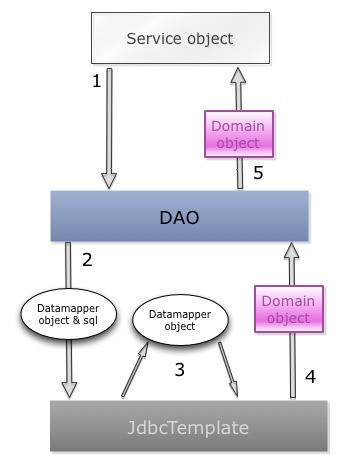
\includegraphics[width=0.5\textwidth]{images/datatier.jpg}
	  \end{center}
	  \caption{Data access pattern in the data tier}  \label{fig:datatier}
	\end{figure} 
shows how object relational mapping is done in the data tier. Here's what happens when the domain logic layer asks the datasource layer to perform a CRUD operation (e.g a Read operation).
		
\begin{enumerate}
\item{} The logic layer calls a CRUD operation on a particular DAO object, for instance \textit{shredDAO.getShredById(int shredId); }
\item{} The DAO class uses a JDBCTemplate instance (provided by Spring) to fix boilerplate setups, such as getting, and closing a database connection. The JDBCTemplate is also responsible for executing the database query itself, provided that it gets a SQL statement from its caller. For instance: 
	\begin{lstlisting}
	@Service
	public class ShredDAOImpl implements ShredDAO {
	
		@Autowired
		private JdbcTemplate jdbcTemplate;
		
		public Shred getShredById(int shredId) {
			String sql =  "SELECT * FROM Shred s,Shredder sr WHERE s.Owner = sr.Id AND s.Id = ?";
			return jdbcTemplate.queryForObject(sql, new Object[]{shredId}, new ShredMapper());
		}
	}	
\end{lstlisting}
\item{} The JDBCTemplate does callbacks to a mapper object provided by the caller. In the above code, the callback calls a function in the ShredMapper class. This class knows how to build a Shred object given the result from a database query that the JDBCTemplate executes. An example of how the ShredMapper class looks like is given below:
Example:
\begin{lstlisting}
public class ShredMapper implements RowMapper <Shred>{
	
	public Shred mapRow(ResultSet rs, int rowNum) throws SQLException {
		Shred shred = this.setConcreteShredder();
		shred.setId(rs.getInt("id"));
		shred.setDescription(rs.getString("Description"));
		shred.setOwner( new ShredderMapper().mapRow(rs, rowNum) );
		// Lots of more mapping ...
		return shred;
	}
}

\end{lstlisting}	
\item{} The domain object created by the mapper is returned from the JDBCTemplate back to the DAO object, which depending on the type of query might catch an exception to provide nice feedback to the service function. An exception might for example be thrown by the DAO if a Shred with the given Id does not exist.
\item{} Finally the DAO function returns the domain object back to the domain logic layer. 
\end{enumerate}	

Clearly, there is a lot of code necessary in order to marshall SQL data. However, the advantage is that the programmer has complete control of how the database results are mapped to Java objects. 

	
\subsection{How Much Data to Fetch}
One issue in the data source layer is to decide how much data to fetch from the database when an object is requested. For instance when a request is made for a Shred, should the DAO function fetch the whole Shred object, fetch the Shred's owner, all the tag objects for the Shred, all the comments and rating etc. This is a tradeoff decision, considering fetching everything requires many SQL joins and much data-mapper processing in Java. These join operations are very performance expensive. But it avoids having to fetch the server for more data at a later point in time, if more of the domain object has to be fetched. One approach is to eagerly fetch every table column and to populate every foreign reference, which would require a large amount of processing, very much data stored in memory, and much data returned back to the client that probably will never be used. The decision I have made is to implement CRUD operations that are customized for the views in the presentation layer. For example, shredders view need a list of Shredders with their profile data, but without their related list of fanees, shreds and battles. Therefore, the SQL read operation used in this case would not eagerly fetch these other tables, but only the Shredder's profile data. On the other hand, if the shredder view is to be rendered, the database will populate the Shredder with all its fanees and all its Shreds. Thus, I have a lot of customized CRUD operations in the data source layer.		

\section{Summary of The Data Source Layer }
The data source layer is responsible for manipulating the database. The database is built with PostgreSQL, where object relational mapping is manually built with Java, instead of using an ORM tool. This requires a lot of Java code, but the code is very flexible and facilitates optimized database marshalling and querying.

\section{Summary}
Architecture 1.0 is a thin-client Java Web app built with a SQL database. All the application's logic happens on the server, where the code is divided into three separate layers; the presentation-, domain logic- and datasource layer. The presentation layer is built with the MVC pattern, in which controller handlers handle HTTP requests, delegates to business operations in the domain logic layer, and upon return, populates a model object with data that is needed to create an HTML page that is sent back to the user. The domain logic layer implements business operations, and delegates persistency handling to the data source layer. The application relies heavily on in-memory Session objects to maintain state. Also, some JavaScript is added to the HTML in order to implement view logic that generates quick and interactive behavior.
		
